\documentclass[11pt,a4paper]{article}
\usepackage{amsmath,amssymb,amsfonts}
\usepackage{mathtools}
\usepackage{bm}
\usepackage{graphicx}
\usepackage{microtype}
\usepackage{hyperref}
\usepackage{cleveref}
\usepackage{booktabs}
\usepackage{natbib}
\usepackage{xcolor}
\usepackage{geometry}
\usepackage{enumitem}
\usepackage{fancyhdr}
\usepackage{array}
\usepackage{multicol}
\usepackage{etoolbox}
\usepackage{titlesec}

% Page layout
\geometry{margin=1in}

% Header and footer
\pagestyle{fancy}
\fancyhf{}
\fancyhead[L]{\textit{PBMA Transition Dynamics}}
\fancyhead[R]{\thepage}
\renewcommand{\headrulewidth}{0.4pt}

% Section styling
\titleformat{\section}
  {\normalfont\Large\bfseries}{\thesection}{1em}{}
\titleformat{\subsection}
  {\normalfont\large\bfseries}{\thesubsection}{1em}{}

% Theorem-like environments
\newtheorem{theorem}{Theorem}[section]
\newtheorem{lemma}[theorem]{Lemma}
\newtheorem{proposition}[theorem]{Proposition}
\newtheorem{corollary}[theorem]{Corollary}
\newtheorem{definition}{Definition}[section]
\newtheorem{remark}{Remark}[section]

% Math operators
\DeclareMathOperator{\E}{\mathbb{E}}
\DeclareMathOperator{\Var}{\text{Var}}
\DeclareMathOperator{\Cov}{\text{Cov}}
\DeclareMathOperator{\argmax}{\arg\!\max}
\DeclareMathOperator{\argmin}{\arg\!\min}

% Title information
\title{\vspace{-1.5cm}\LARGE\textbf{Transition Dynamics in the PBMA Aiyagari Model}}
\date{\today}

\begin{document}

\maketitle

\begin{abstract}
\noindent
\begin{enumerate}
    \item Use Mukoyama's approach for computing transitions between steady states
    \item From SRPE to CPE: Gradual adjustment and converge.
    \item From CPE to SRPE: do not converge
    \item We use Monte Carlo method to simulate the Mixed Action Equilibrias. 
\end{enumerate}
\end{abstract}

\section{Model Specification}

\subsection{Households}

Households are infinitely lived with two distinct discount factors:
\begin{itemize}
    \item Short-run discount factor $\beta\delta \in (0,1)$
    \item Long-run discount factor $\delta \in (0,1)$
\end{itemize}

\noindent The household optimization problem is:
\begin{align}
\max_{\{c_t\}_{t\geq 0}} \E\left[u(c_0) + \beta \sum_{t=1}^{\infty} \delta^t u(c_t)\right]
\end{align}

\noindent Subject to the budget constraint:
\begin{align}
a_{t+1} + c_t &\leq wz_t + (1 + r)a_t\\
c_t &\geq 0\\
a_t &\geq -B
\end{align}

\noindent Where $c_t$ is consumption, $a_t$ is asset holdings, $z_t$ is an exogenous component of labor income capturing stochastic employment risk, $w$ is the wage, $r$ is the interest rate, and $B$ is the borrowing constraint.\\
\\
\noindent We assume log utility $u(c) = \ln(c)$ and that labor productivity follows a Markov process with transition matrix $\Pi$ and state space $\{z_1, z_2, \ldots, z_n\}$.

\subsection{Firms}

\noindent Production occurs according to a Cobb-Douglas technology:
\begin{align}
Y = AK^\alpha N^{1-\alpha}
\end{align}

\noindent Firms maximize profits by choosing capital and labor:
\begin{align}
\max_{K,N} \{AK^\alpha N^{1-\alpha} - (r+\eta)K - wN\}
\end{align}

\noindent The first-order conditions yield:
\begin{align}
r &= A\alpha\left(\frac{N}{K}\right)^{1-\alpha} - \eta\\
w &= A(1-\alpha)\left(\frac{K}{N}\right)^{\alpha}
\end{align}

\section{Equilibrium Concepts}

There are three types of equilibrium concepts:

\begin{itemize}
    \item Agents keep using short-run policy $\implies$ Short-Run Policy Equilibrium (SRPE)
    \item Agents Keep using continuation policy $\implies$ Continuation Policy Equilibrium (CPE)
    \item Agents keep mixing these two policies $\implies$ PBMA equilibrium.
\end{itemize}

\noindent \textbf{Remark}: The PBMA equilibrium is constructed numerically. And it will be discussed separately in Section 4.

\subsection{Computation Algorithm}
Here is the outline of our algorithm:
\begin{enumerate}
    \item Compute the optimal continuation policy $\sigma_c$ and continuation value $v_c$ by solving the following Bellman equation with discount factor $\delta$
    $$
    v_c(a,z) = \max_{a' \in \Gamma(a,z)} \left\{u(wz + (1+r)a - a') + \delta \sum_{z'} v_c(a',z')\Pi(z,z')\right\}
    $$
    using Howard Policy Iteration
    \item Compute the short-run policy $\sigma_s$ and lifetime value $v_s$ by solving a two-period DP problem as follows with discount factor $\beta\delta$
    $$
    v_s (a,z) = \max_{a'\in\Gamma(a,z)} \left\{u(wz + (1+r)a - a') + \beta\delta \sum_{z'} v_c(a',z')\Pi(z,z') \right\}
    $$
    \item Compute the equilibriums using standard algorithm to find the equilibrium aggregate capital for solely using short-run policy and solely using continuation policy for further analysis. 
\end{enumerate}

\subsection{Comparing the Aggregate Capital}
\noindent For our baseline calibration ($\beta=0.5$, $\delta=0.96$, $\alpha=0.33$, $\delta=0.05$), we compute:
\begin{align}
K_{SRPE} &= 3.89\\
K_{CPE} &= 8.09
\end{align}

\noindent And we varies the value of $\beta = 0, 0.1, 0.2, \cdots, 0.9, 1$ and compute the aggregate equilibrium capital. Here is the plot

\subsection{Comparing the Stationary Asset Distribution}
Here is the plot for different stationary asset distribution  with $\beta = 0, 0.1, 0.2, \cdots, 0.9, 1$
\section{Transition Dynamics Methodology}
We adapt Mukoyama's methodology to compute transitions between these equilibria.\\
\\
First, we discuss the transition path from SRPE to CPE, i.e., agents is originally at SRPE and then there is a sudden change in the discount factor $\beta$ to 1.\\
\\
Second, we discuss the transition path from CPE to SRPE, i.e., agents are originally at CPE and then there is a sudden change in the discount factor $\beta$  from  1 to some lower value.\\
\\

\noindent The algorithm proceeds as follows:

\begin{enumerate}
    \item Compute initial steady state capital $K^s$ and terminal steady state capital $K^c$
    \item Guess a time series for capital $\{K_t\}_{t=1}^T$ where $T$ is sufficiently large
    \item Derive prices $\{r_t,w_t\}_{t=1}^T$ from firm's optimization conditions
    \item Use backward induction to compute value functions and policy functions for each period
    \item Simulate the economy forward starting from the initial distribution
    \item Compare the implied capital path to the initial guess and update
    \item Iterate until convergence
\end{enumerate}

\subsection{Backward Induction}

For the transition from SRPE to CPE, we:
\begin{enumerate}
    \item Start with terminal value function $v_T = v_c$
    \item For $t = T-1, T-2, \ldots, 1$, we solve a two-period DP problem 
        \begin{align}
            v_t(a,z) = \max_{a'} \{u(w_tz + (1+r_t)a - a') + \delta\sum_{z'} v_{t+1}(a',z')\Pi(z,z')\}
        \end{align}
    \item Store the resulting policy functions $\sigma_t(a,z)$
\end{enumerate}

\noindent For the transition from CPE to SRPE, the backward induction use $v_s$ as terminal value function and uses the short-run discount factor $\beta\delta$ between periods $t$ and $t-1$.

\subsection{Forward Simulation}

Starting with the initial stationary distribution $\psi_0$:
\begin{enumerate}
    \item For $t = 1, 2, \ldots, T-1$:
        \begin{align}
            \psi_t(a',z') = \sum_{a,z} \mathbb{I}[a' = \sigma_{t-1}(a,z)]\psi_{t-1}(a,z)\Pi(z,z')
        \end{align}
    \item Compute aggregate capital for each period:
        \begin{align}
            K_t = \sum_{a,z} a \cdot \psi_t(a,z)
        \end{align}
\end{enumerate}
\subsection{Transition dynamics from SRPE to CPE}
The above algorithm converges and we can find a smooth transition path from SRPE to CPE. The transition path is plotted below with different beta.

\subsection{Transition dynamics from CPE to SRPE}
Does not converge. By backward induction, the aggregate capital drops to zero very quickly.\\
\\
This might be possible, as keep using short-run policy is unstable.  Here is the illustrative plot. I get this plot by setting a larger tolerance.

\section{PBMA}
This section discuss PBMA in this model. We let $\omega$ be the probability of using the short-run policy.
\subsection{Stationary Asset Distribution of PBMA}
Since we can get the Markov matrix for both policies, we can also obtain the Markov matrix for the PBMA policies as a weighted average. This induces a stationary asset distribution for PBMA policies and a corresponding aggregate capital. Here is a plot for the aggregate capital under different $\omega$.
\begin{figure}[h!]
    \centering
    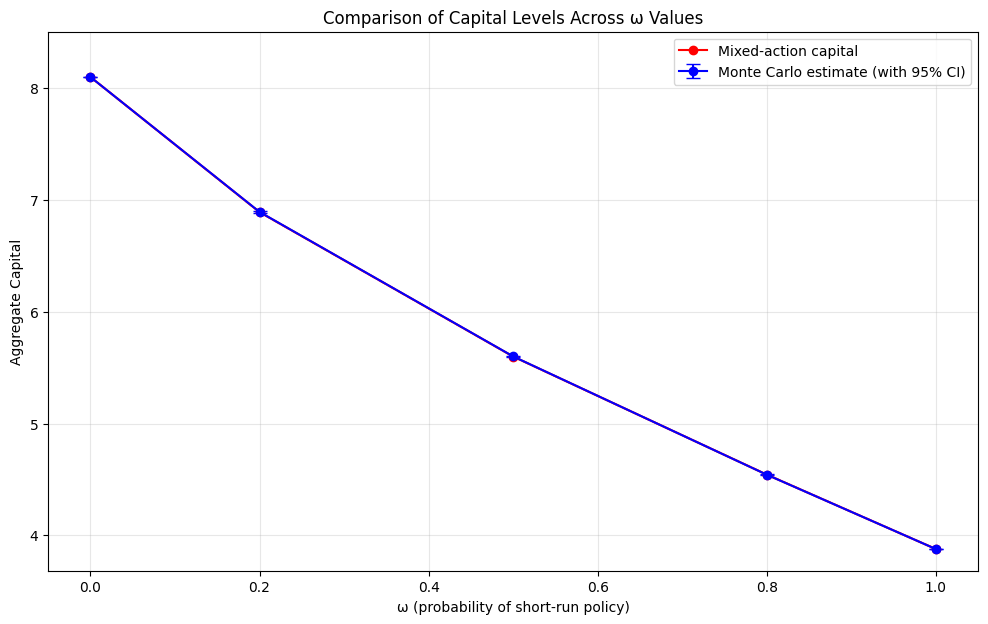
\includegraphics[width=1\linewidth]{QHD/image/pbma_capital.png}
    \caption{PBMA aggregate capital across $\omega$}
\end{figure}

\subsection{Use Monte Carlo to verify}

Then I use Monte Carlo method to verify. The general procedure is as follows:



\subsection{Result of Monte Carlo}

As shown in the previous figure, at every level, the simulation result is very similar to the one from stationary asset distribution of PBMA. Here is a detailed result for $\omega=0.2$. (Under other $\omega$, the result is similar)
\begin{figure}[h!]
    \centering
    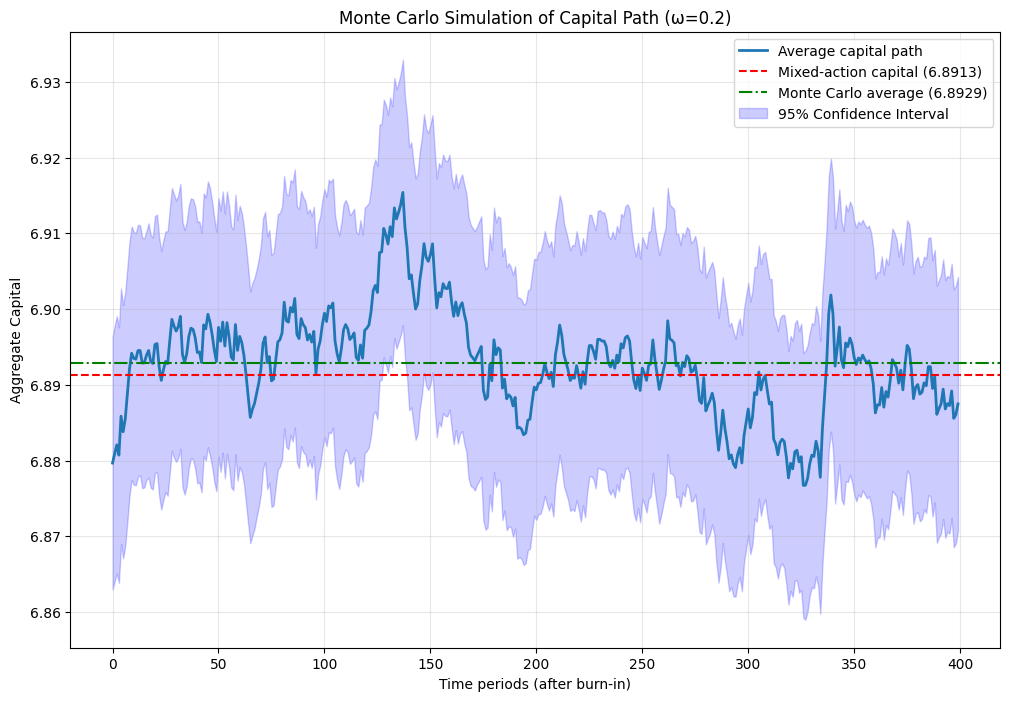
\includegraphics[width=1\linewidth]{QHD/image/mc_2.png}
    \caption{Simulation Result for $\omega=0.2$}
\end{figure}

\begin{figure}[h!]
    \centering
    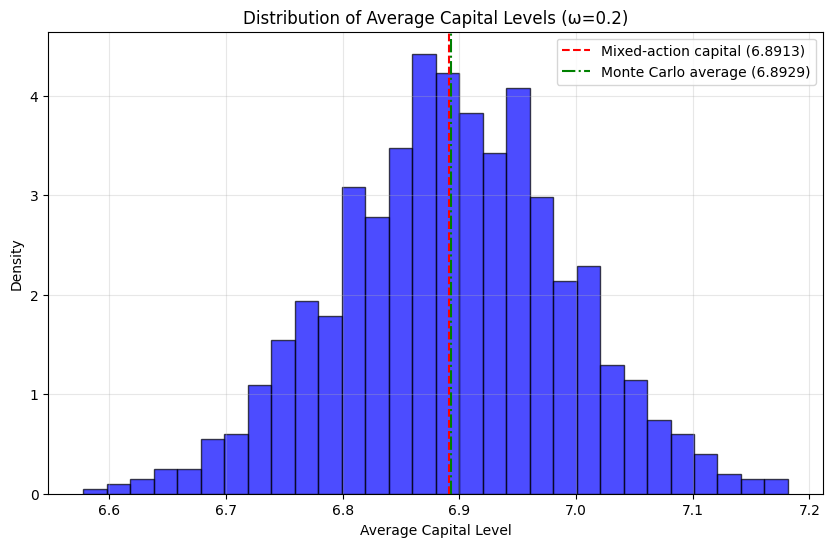
\includegraphics[width=1\linewidth]{QHD/image/mc_dist_2.png}
    \caption{Simulation Distribution for $\omega=0.2$}
\end{figure}

\section{Asset Distribution Dynamics}
Here is a plot of asset distribution dynamics. 


\newpage

\bibliographystyle{econometrica}
\begin{thebibliography}{9}

\bibitem{aiyagari1994}
Aiyagari, S. Rao (1994).
\newblock ``Uninsured Idiosyncratic Risk and Aggregate Saving.''
\newblock \textit{Quarterly Journal of Economics}, 109(3): 659--684.

\bibitem{mukoyama}
Mukoyama, Toshihiko.
\newblock ``Transition Dynamics in the Aiyagari Model, with an application to Wealth Tax.''
\newblock Working Paper.

\end{thebibliography}

\end{document}